\documentclass[12pt,pdf,hyperref={unicode}]{beamer}


%\documentclass[10pt]{beamer}

\usetheme[progressbar=frametitle]{metropolis}

\usepackage{booktabs}
\usepackage[scale=2]{ccicons}

\usepackage{pgfplots}
\usepgfplotslibrary{dateplot}

\usepackage{xspace}
\newcommand{\themename}{\textbf{\textsc{metropolis}}\xspace}


%\usepackage{lmodern}

% подключаем кириллицу 
\usepackage[T2A]{fontenc}
\usepackage[utf8]{inputenc}
\usepackage{listings}
%\usepackage{graphicx}
\usepackage{hyperref}

% отключить клавиши навигации
\setbeamertemplate{navigation symbols}{}

% тема оформления
\usetheme{Pittsburgh}

% цветовая схема
\usecolortheme{default}

\definecolor{light-gray}{gray}{0.90}

\title{Семинар №8}   
\subtitle{ФАКИ \the\year}
\author{Бирюков В. А.} 
\date{\today}
% \logo{
\includegraphics[height=5mm]{images/logo.png}\vspace{-7pt}}

\begin{document}

\lstset{language=C}

% титульный слайд
\begin{frame}
\titlepage
\end{frame} 

\defverbatim[colored]\makeset{
\begin{lstlisting}[language=C++,basicstyle=\ttfamily,keywordstyle=\color{blue}]
void make_set(int X) {
  parent[X] = X;
}
\end{lstlisting}
}

\lstset{
  language=C,                % choose the language of the code
  basicstyle=\ttfamily,
  columns=fixed,
  fontadjust=true,
  basewidth=0.5em,
  keywordstyle=\color{blue}\bfseries,
  commentstyle=\color{gray},
  stringstyle=\ttfamily\color{yellow!40!red},
  showstringspaces=false,
  %numbers=false,                   % where to put the line-numbers
  numbersep=5pt,
  numberstyle=\tiny\color{gray},
  numberfirstline=true,
  stepnumber=1,                   % the step between two line-numbers.        
  numbersep=5pt,                  % how far the line-numbers are from the code
  backgroundcolor=\color{white!90!gray},  % choose the background color. You must add \usepackage{color}
  showstringspaces=false,         % underline spaces within strings
  captionpos=b,                   % sets the caption-position to bottom
  breaklines=true,                % sets automatic line breaking
  breakatwhitespace=true,         % sets if automatic breaks should only happen at whitespace
}
\lstset{literate=%
   *{0}{{{\color{red!20!violet}0}}}1
    {1}{{{\color{red!20!violet}1}}}1
    {2}{{{\color{red!20!violet}2}}}1
    {3}{{{\color{red!20!violet}3}}}1
    {4}{{{\color{red!20!violet}4}}}1
    {5}{{{\color{red!20!violet}5}}}1
    {6}{{{\color{red!20!violet}6}}}1
    {7}{{{\color{red!20!violet}7}}}1
    {8}{{{\color{red!20!violet}8}}}1
    {9}{{{\color{red!20!violet}9}}}1
}

\section{Указатели}

\begin{frame}[fragile]
\frametitle{Адрес переменной} 
У каждой переменной есть адрес -- номер ячейки памяти.
\begin{center}
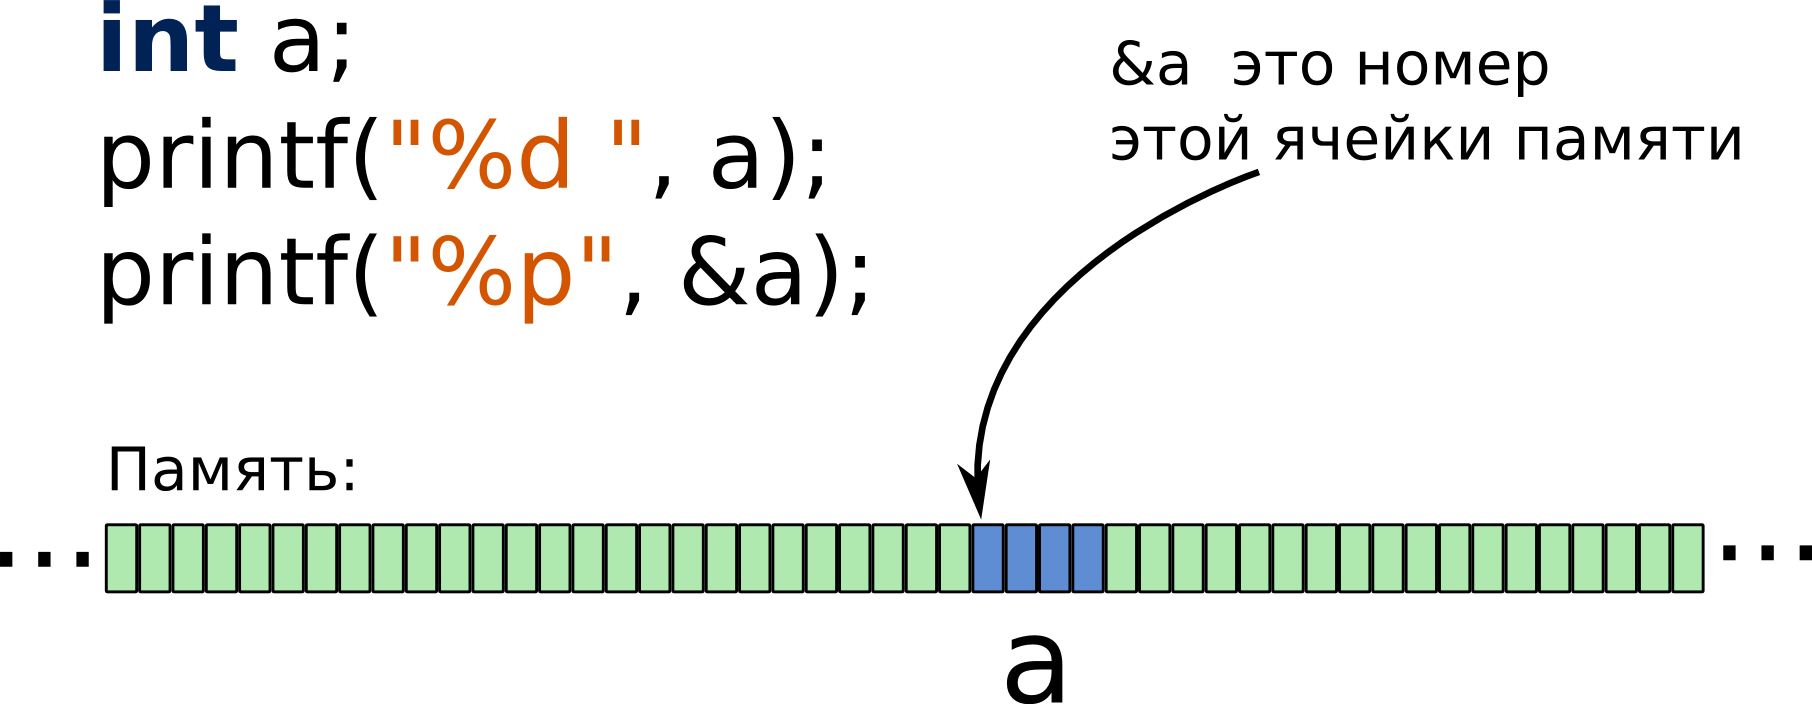
\includegraphics[width=0.95\linewidth]{images/variable_address.png}
\end{center}
\end{frame}


\begin{frame}[fragile]
\frametitle{Указатели} 
\framesubtitle{Указатели в памяти, объявление указателей}
Указатель -- это переменная, которая хранит адреса. 
Размер указателя = 8 байт в 64-х битных системах.
\begin{center}
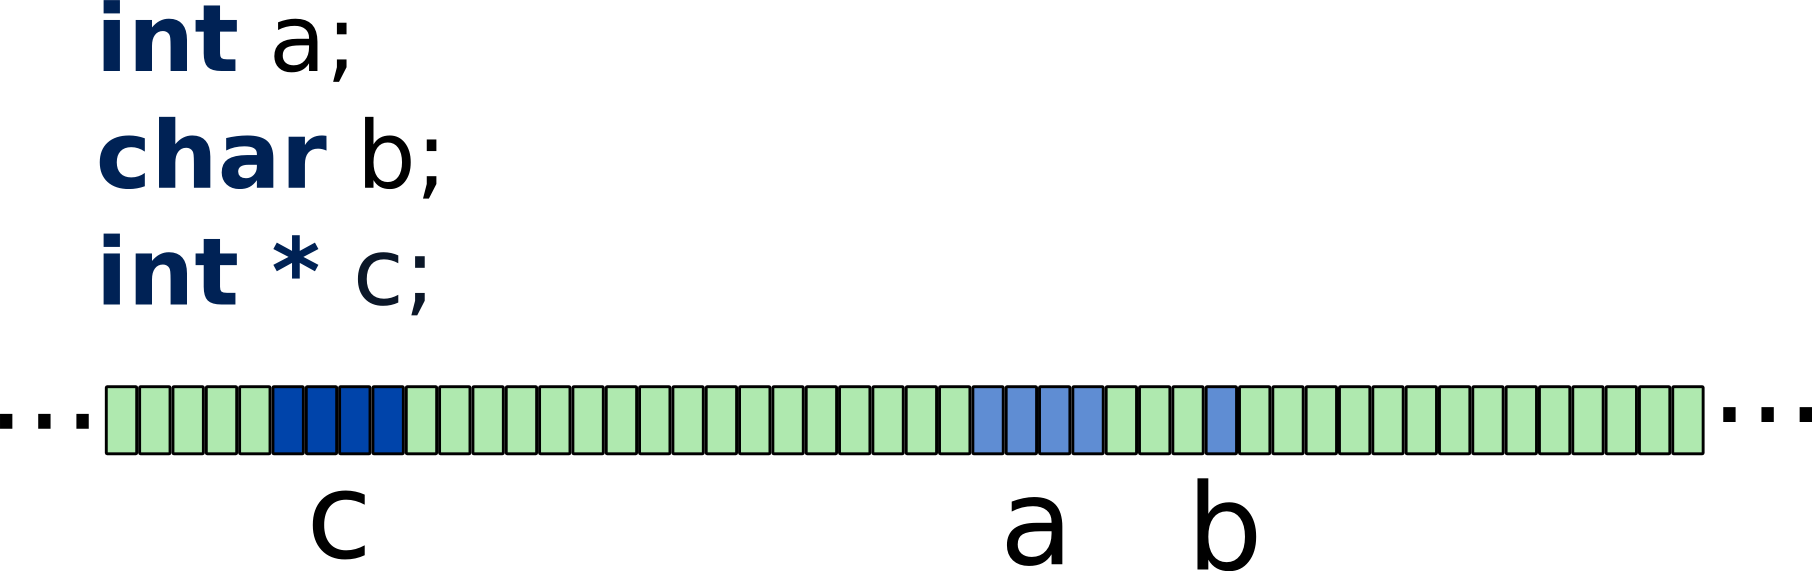
\includegraphics[width=0.95\linewidth]{images/memory_pointer_1.png}
\end{center}
\end{frame}

\begin{frame}[fragile]
\frametitle{Указатели} 
\framesubtitle{Указатели в памяти, объявление указателей}
Указатель -- это переменная, которая хранит адреса. 
Размер указателя = 8 байт в 64-х битных системах.
\begin{center}
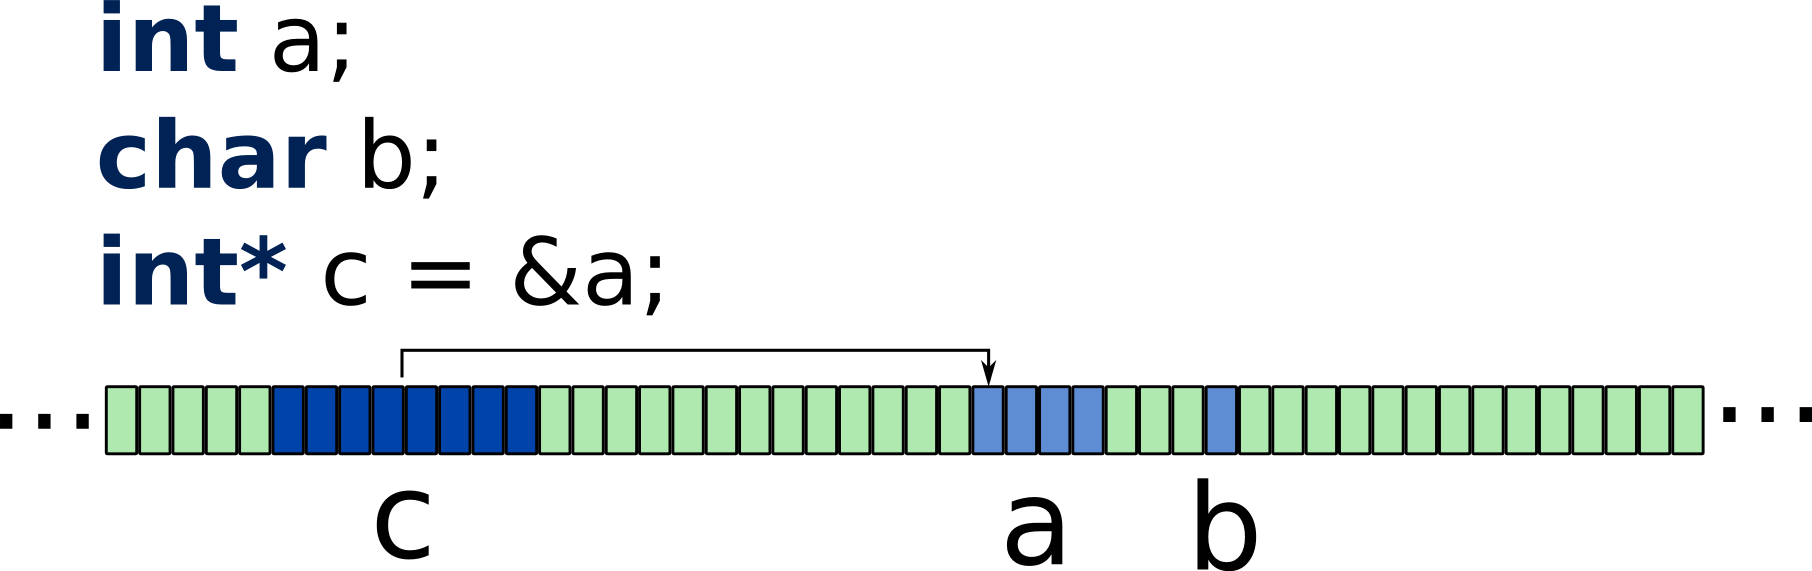
\includegraphics[width=0.95\linewidth]{images/memory_pointer_2.png}
\end{center}
\end{frame}

\begin{frame}[fragile]
\frametitle{Указатели} 
\framesubtitle{Указатели в памяти, объявление указателей}
Указатель -- это переменная, которая хранит адреса. 
Размер указателя = 8 байт в 64-х битных системах.
\begin{center}
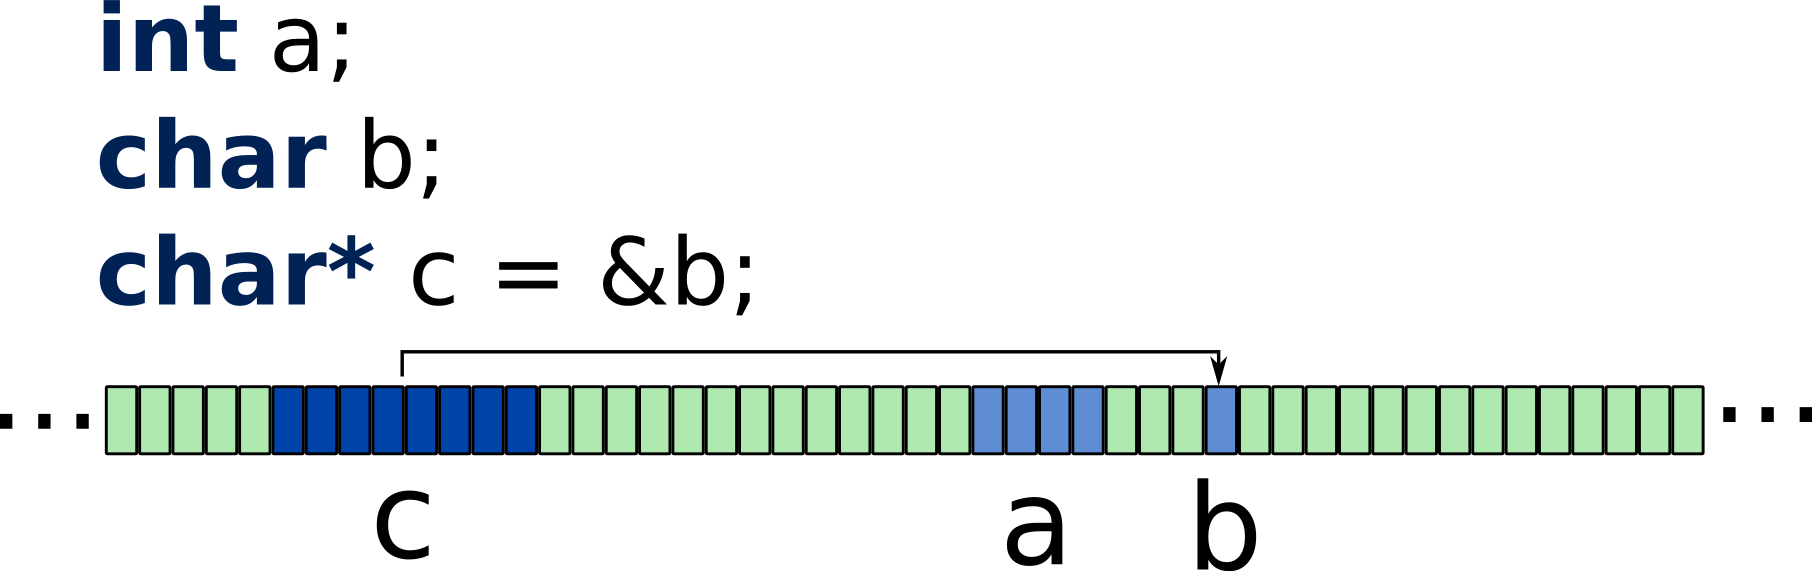
\includegraphics[width=0.95\linewidth]{images/memory_pointer_3.png}
\end{center}
\end{frame}

\begin{frame}[fragile]
\frametitle{Указатели} 
\framesubtitle{Указатели в памяти, объявление указателей}
Указатель -- это переменная, которая хранит адреса. 
Размер указателя = 8 байт в 64-х битных системах.
\begin{center}
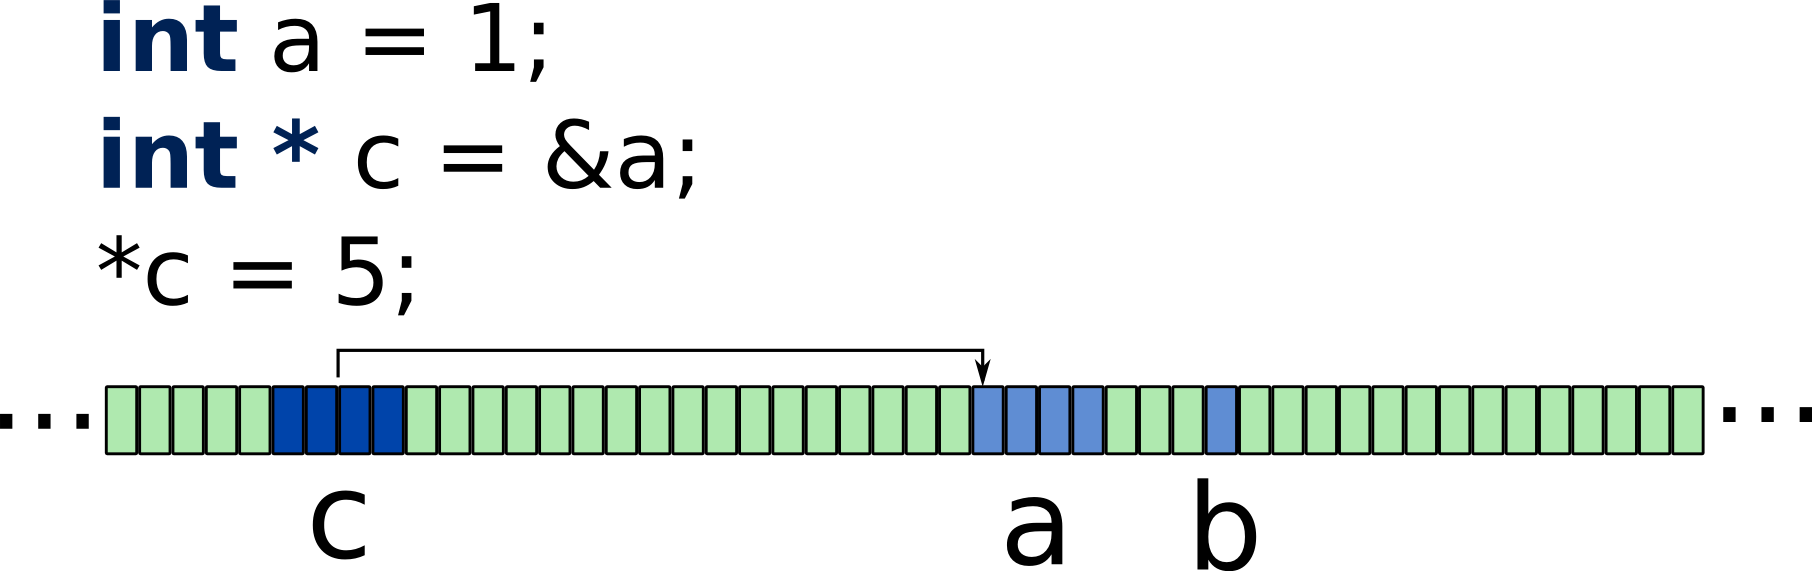
\includegraphics[width=0.95\linewidth]{images/memory_pointer_4.png}
\end{center}
\end{frame}


\section{Передача аргументов в функцию}

\begin{frame}[fragile]
\frametitle{Передача аргументов в функцию}
\framesubtitle{Передача по значению}
\begin{lstlisting}
int min(int a, int b)
{
    if (a < b)
        b = a;
   	return b;
}
int main()
{
    int a = 10, b = 40;
    int c = min(a, b);
    printf("%d\n", b);
}
\end{lstlisting}
\end{frame}

\begin{frame}[fragile]
\frametitle{Передача аргументов в функцию}
\framesubtitle{Передача по значению}
\begin{lstlisting}
int min(int a, int b)
{
    if (a < b)
        b = a;
   	return b;
}
int main()
{
    int x = 10, y = 40;
    int c = min(x, y);
    printf("%d\n", y);
}
\end{lstlisting}
\end{frame}

\begin{frame}[fragile]
\frametitle{Передача аргументов в функцию}
\framesubtitle{Передача по значению}
\begin{lstlisting}
int min(int a, int b)
{
    if (a < b)
        b = a;
   	return b;
}
int main()
{

    int c = min(10, 40);

}
\end{lstlisting}
\end{frame}

\begin{frame}[fragile]
\frametitle{Передача аргументов в функцию}
\framesubtitle{Передача с помощью указателей}
\begin{lstlisting}
void normalize(float* a, float* b)
{
    float sum = *a + *b;
    *a = *a / sum;
    *b = *b / sum;
}
int main()
{
    float x = 10.0, y = 40.0;
    normalize(&x, &y);
    printf("%f\n", y);
}
\end{lstlisting}
\end{frame}


\begin{frame}[fragile]
\frametitle{Функция swap()} 
\framesubtitle{Передача по значению}
\begin{center}
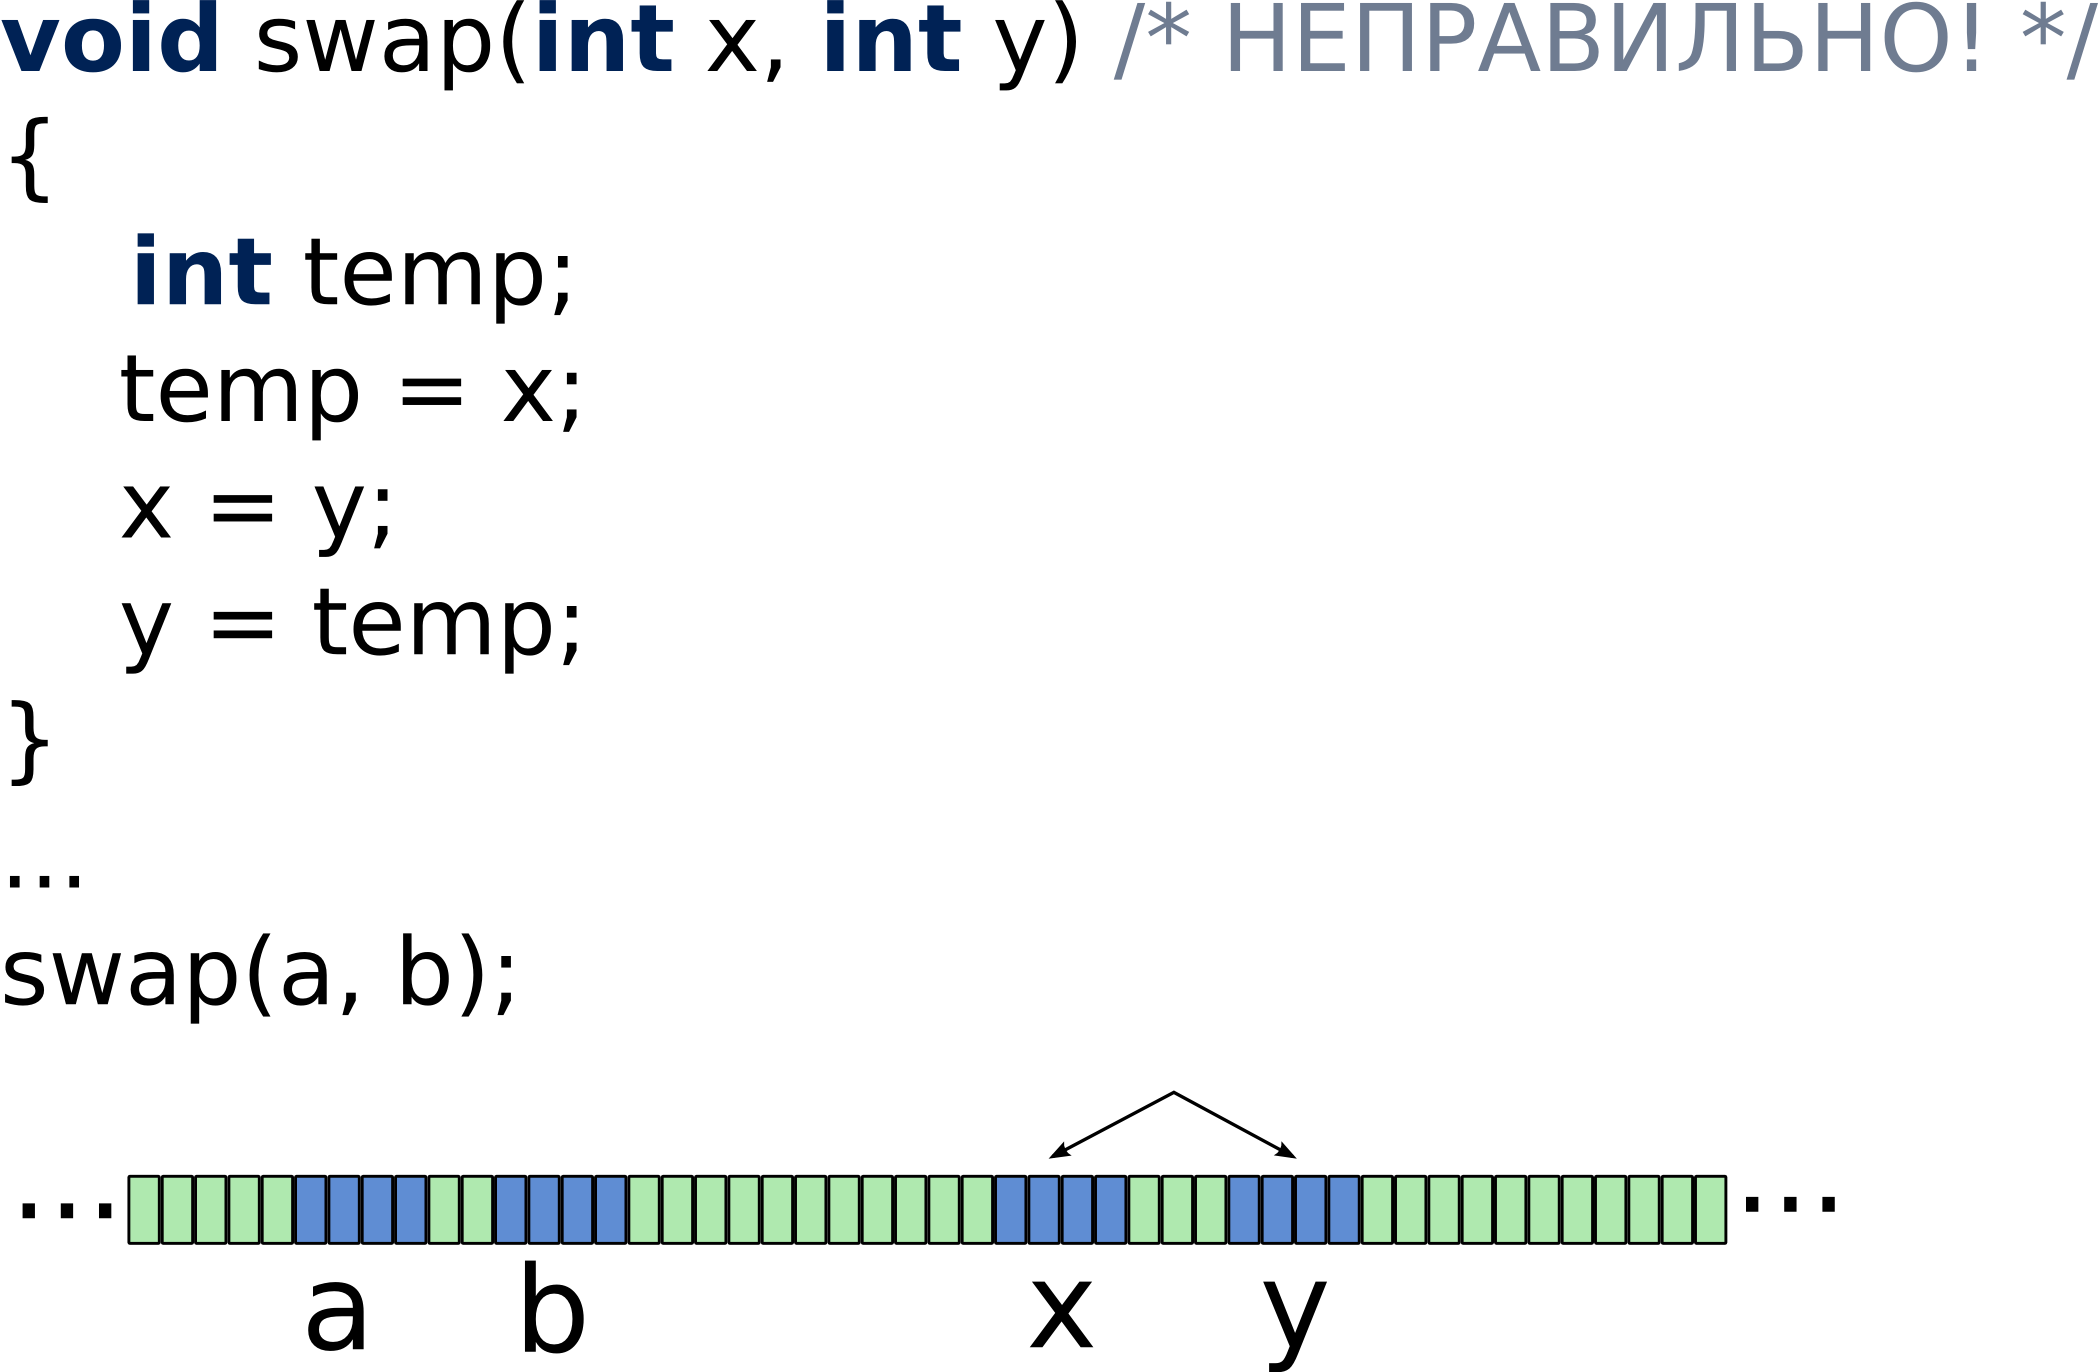
\includegraphics[height=0.55\linewidth]{images/swap_wrong.png}
\end{center}
\end{frame}

\begin{frame}[fragile]
\frametitle{Функция swap()} 
\framesubtitle{Передача по адресу}
\begin{center}
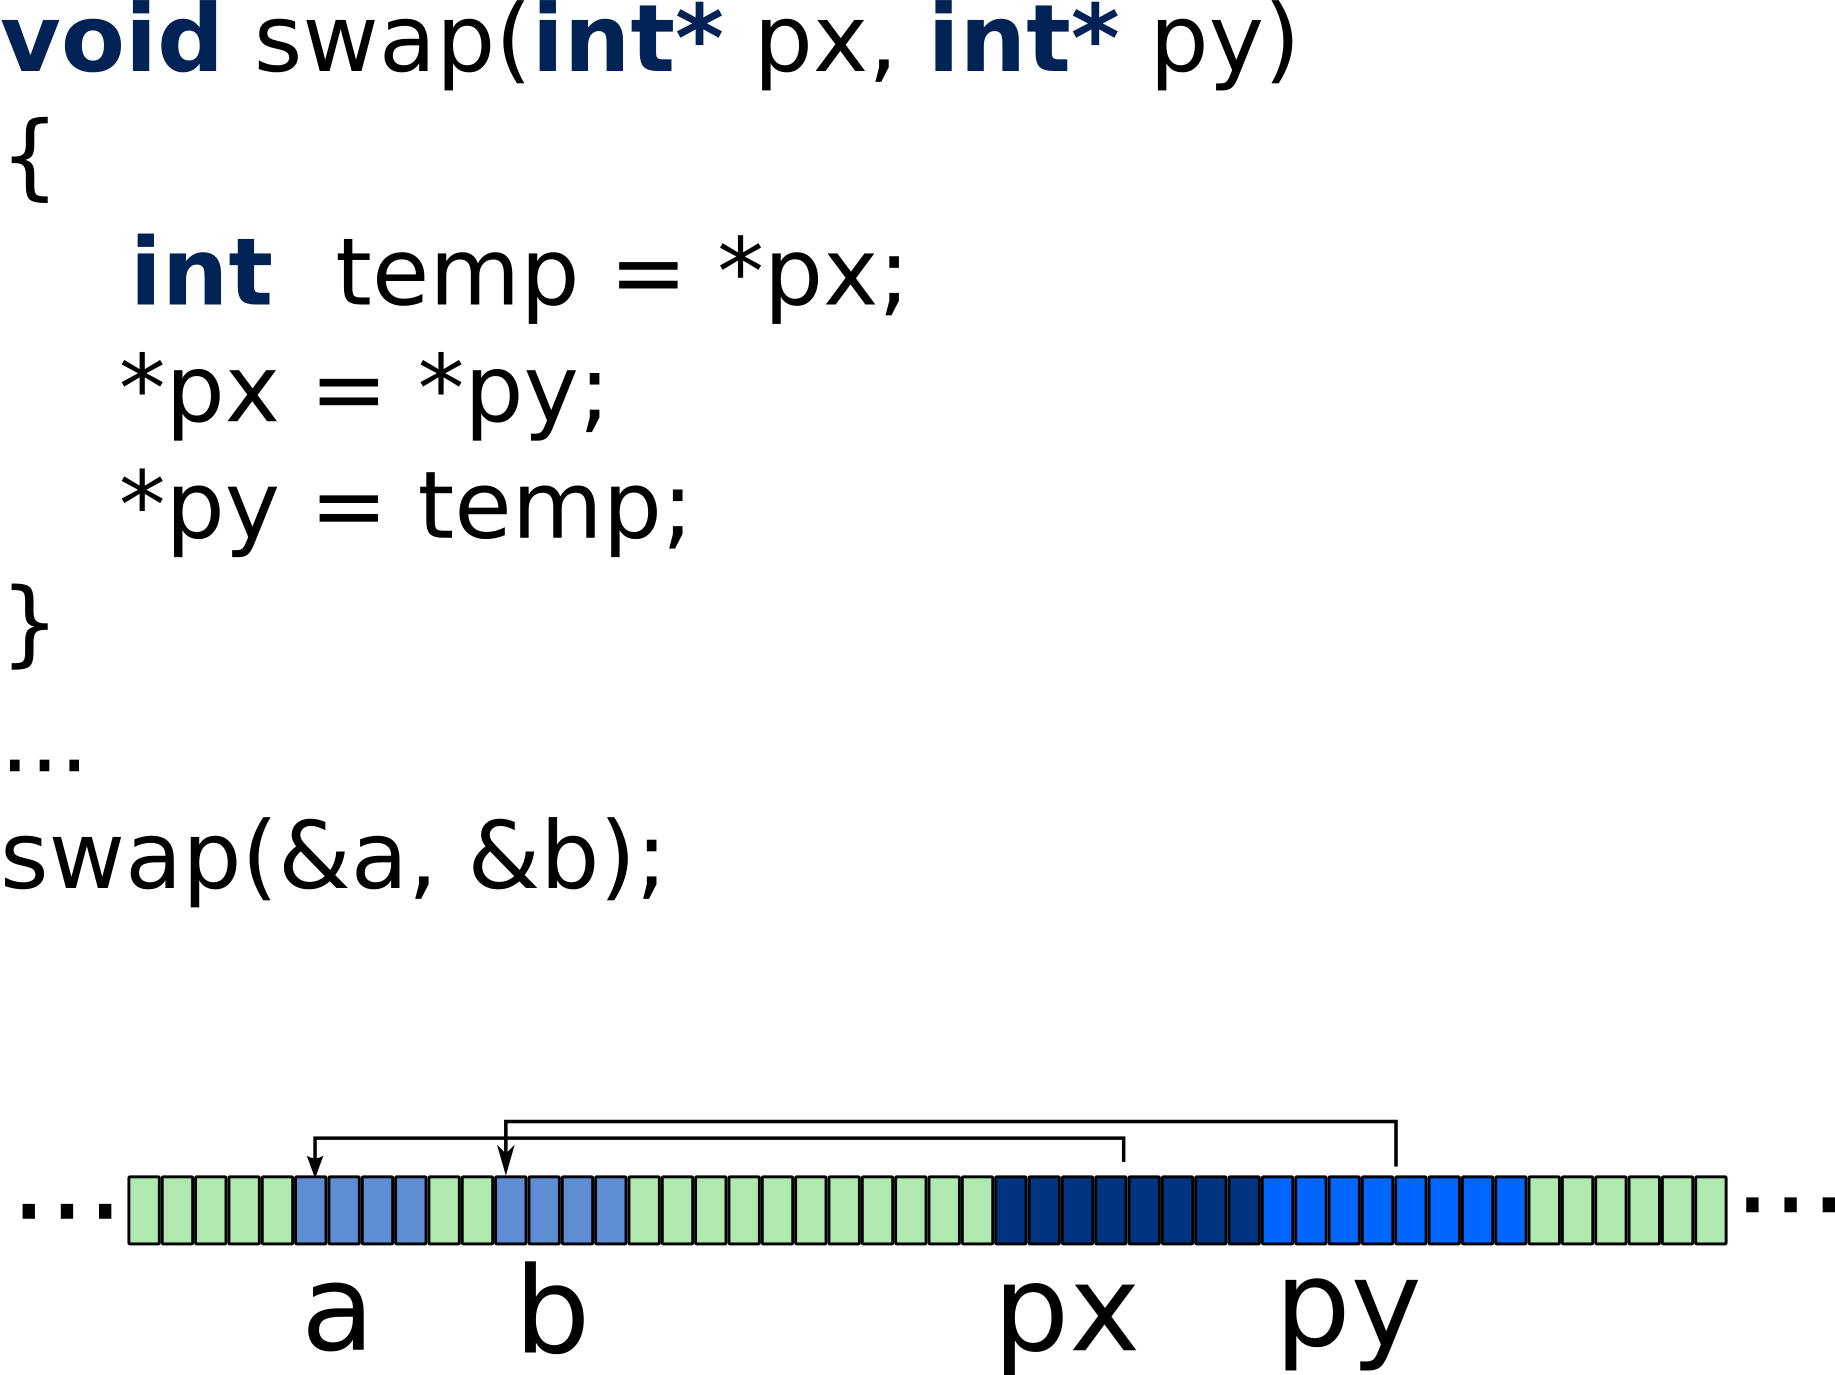
\includegraphics[height=0.55\linewidth]{images/swap_right.png}
\end{center}
\end{frame}

\begin{frame}[fragile]
\frametitle{Передача массивов в функцию}
\framesubtitle{Автоматически передаются с помощью указателей}
\begin{lstlisting}
void add_num(int n, int arr[], int x)
{
    for (int i = 0; i < n; ++i)
        arr[i] += x;
}
int main()
{
    int arr[5] = {1, 5, 7, 3, 16};
    add_num(5, arr, 2);
}
\end{lstlisting}
\end{frame}

\begin{frame}[fragile]
\frametitle{Передача массивов в функцию}
\framesubtitle{Автоматически передаются с помощью указателей}
\begin{lstlisting}
void add_num(int n, int* arr, int x)
{
    for (int i = 0; i < n; ++i)
        arr[i] += x;
}
int main()
{
    int arr[5] = {1, 5, 7, 3, 16};
    add_num(5, arr, 2);
}
\end{lstlisting}
\end{frame}


\begin{frame}[fragile]
\frametitle{Указатели}
\framesubtitle{Итого}
\begin{itemize}
\item Каждая переменная имеет адрес -- номер ячейки памяти
\item Указатель -- это переменная, которая хранит адреса
\item Обычные параметры передаются в функцию по значению
\item Чтобы можно было изменять переменные в функциях нужно передавать указатели
\item Массивы всегда передаются через указатели
\end{itemize}
\end{frame}


\section{Директивы и typedef}
\begin{frame}[fragile]
\frametitle{Директивы \#include и \#define} 
\begin{center}
\begin{itemize}
\item \textbf{\#include} — вставляет текст из указанного файла, например:
\begin{verbatim}
#incude <stdio.h>
\end{verbatim}
Находит файл stdio.h и вставляет за место этой строчки.
\item \textbf{\#define} — задаёт макрос или символическую константу
\begin{verbatim}
#define SIZE 100
\end{verbatim}
Перед компиляцией заменяет в тексте SIZE на 100
\end{itemize}
\end{center}
\end{frame}


\begin{frame}[fragile]
\frametitle{Typedef} 
\begin{itemize}
\item Typedef -- ключевое слово в языке C \\
\item Используется для того, чтобы дать типу новое имя \\
\item 
\begin{lstlisting}[language=C++,basicstyle=\ttfamily,keywordstyle=\color{blue}]
typedef int my_new_int;
\end{lstlisting}
\item 
\begin{lstlisting}[language=C++,basicstyle=\ttfamily,keywordstyle=\color{blue}]
typedef unsigned long long ull;
\end{lstlisting}
\end{itemize}
\end{frame}




\section{Структуры}
\begin{frame}[fragile]
\frametitle{Структуры} 
\begin{itemize}
\item Структура -- это композитный тип данных, группирующий, без сокрытия набор значений \\
\item 
\begin{lstlisting}[language=C++,basicstyle=\ttfamily,keywordstyle=\color{blue}]
struct book 
{
   char title[50];
   int pages;
   float price;
};
\end{lstlisting}
\begin{verbatim}
int a;         // Объявление int 
struct book b; // Объявление структуры book 
\end{verbatim}
\end{itemize}
\end{frame}


\begin{frame}[fragile]
\frametitle{Структуры} 
\framesubtitle{Пример} 
Инициализация структуры:
\begin{lstlisting}[language=C++,basicstyle=\ttfamily,keywordstyle=\color{blue}]
struct book b1 = {"Don Quixote", 710, 900.0};
struct book b2 = {"War and Peace", 1500, 1200.0};
struct book b3 = {"The Dark Tower", 300, 500.0};
\end{lstlisting}
Доступ к элементу структуры(оператор .):
\begin{lstlisting}[language=C++,basicstyle=\ttfamily,keywordstyle=\color{blue}]
printf("%s costs %.2f R", b1.title, b1.price);
b3.price += 1000.0;
\end{lstlisting}
\end{frame}


\begin{frame}[fragile]
\frametitle{Typedef для структур} 
\begin{itemize}
\item Typedef -- используется для того, чтобы дать типу новое имя \\
\item 
\begin{lstlisting}[language=C++,basicstyle=\ttfamily,keywordstyle=\color{blue}]
typedef struct book Book;
\end{lstlisting}
\item 
\begin{lstlisting}[language=C++,basicstyle=\ttfamily,keywordstyle=\color{blue}]
Book b1 = {"Don Quixote", 710, 900.0};
Book b2 = {"War and Peace", 1500, 1200.0};
Book b3 = {"The Dark Tower", 300, 500.0};
\end{lstlisting}
\end{itemize}
\end{frame}




\begin{frame}[fragile]
\frametitle{Структуры и функции} 
\framesubtitle{Передача структур по значению} 
Структуры передаются по значению, как и обычные переменные:
\begin{lstlisting}[language=C++,basicstyle=\ttfamily,keywordstyle=\color{blue}]
void print_book_info(Book b)
{
    printf("Book info:\n");
    printf("Title: %s\n", b.title);
    printf("Pages: %d\n", b.pages);
    printf("Price: %f\n", b.price);
}
\end{lstlisting}
\end{frame}


\begin{frame}[fragile]
\frametitle{Структуры и функции} 
\framesubtitle{Передача структур с помощью указателей} 
Два варианта работы с указателем на структуру: \\
\begin{lstlisting}[language=C++,basicstyle=\ttfamily,keywordstyle=\color{blue}]
void change_price(Book* b, float new_price)
{
    (*b).price = new_price;
}
\end{lstlisting}
\begin{lstlisting}[language=C++,basicstyle=\ttfamily,keywordstyle=\color{blue}]
void change_price(Book* b, float new_price)
{
    b->price = new_price;
}
\end{lstlisting}
\end{frame}

\begin{frame}[fragile]
\frametitle{Массивы структур} 
\begin{lstlisting}[language=C++,basicstyle=\ttfamily,keywordstyle=\color{blue}]
Book wnp = {"War and Peace", 1500, 1200.0};
Book scifi_books[100] = {
        {"The Dark Tower", 300, 500.0}, 
        {"Fahrenheit 451", 400, 700.0},
        {"The Day of the Triffids", 304, 450.0}
};
scifi_books[3] = wnp;

change_price(&scifi_books[0], 1200.0);
print_book_info(scifi_books[0]);

\end{lstlisting}
\end{frame}

%E9C6AF
%C6E9AF

\end{document}
